% Chapter Template

\chapter{Exercices} % Main chapter title

\label{Chapitre 2} % Change X to a consecutive number; for referencing this chapter elsewhere, use \ref{ChapterX}

\lhead{ \emph{HMM Training and tests}} % Change X to a consecutive number; this is for the header on each page - perhaps a shortened title

%----------------------------------------------------------------------------------------
%	SECTION 1
%----------------------------------------------------------------------------------------
\section{Problèmes à résoudre}

\subsection{c) Compléter le tableau ci-dessus et effectuer les modifications des scripts comme indiqué}

Nous effectuons les modifications du script et analysons les mots ainsi que les enregistrements réalisés.

\begin{tabular}{|c|c|c|c|c|}
\hline 
Mot & Transcription phonétique & N & durée [ms] & n vect acoust \\ 
\hline 
un & œ & 5 & 1168 & 145 \\ 
\hline 
deux & dø & 6 & 994 & 122 \\ 
\hline 
trois & trwa & 8 & 1110 & 137 \\ 
\hline 
quatre & katr & 8 & 1164 & 144 \\ 
\hline 
cinq & sÊk & 7 & 1222 & 151 \\ 
\hline 
peu & pø & 6 & - & - \\ 
\hline 
\end{tabular}

\subsection{d) Entraîner les modèles des 5 chiffres (1-5) avec le script train test hmm.m.}

Nous avons entraîné nos HMM avec le code suivant.

\begin{lstlisting}
N=5; 
A=inittran(N); [MI,SIGMA]=initemis(c1_1,N); 
[NEWA, NEWMI, NEWSIGMA, Ptot] = vit_reestim (c1_1,c1_2,c1_3, A, MI, SIGMA);
disp(['Ptot pour chiffre 1 = 1t' num2str(Ptot)]);
for iter=1:5
   [NEWA,NEWMI,NEWSIGMA,Ptot] = vit_reestim (c1_1,c1_2,c1_3, NEWA, NEWMI, SIGMA);  
   disp(['Ptot pour chiffre 1 = 1t' num2str(Ptot)]);
   %Ptot
end
A1=NEWA; MI1=NEWMI; SIGMA1=SIGMA;
\end{lstlisting}

\subsection{e) Observez l'évolution de la probabilité Ptot lors des itérations d'entraînement pour chaque chiffre. Que pouvez-vous conclure de cette évolution ?}

Lors de l'entainement des HMM, l'évolution des probabilités Ptot sont les suivantes.
\\

\begin{tabular}{|c|c|c|c|c|c|}
\hline 
Iteration & Chiffre un & Chiffre deux & Chiffre trois & Chiffre quatre & Chiffre cinq \\ 
\hline 
1 & -1688.9798 & -1598.4164 & -1504.5904 & -1668.4481 & -1849.6596 \\ 
\hline 
2 & -1469.9455 & -1380.7751 & -1321.3925 & -1442.223 & -1610.0635 \\ 
\hline 
3 & -1467.7647 & -1380.435 & -1317.6448 & -1423.1129 & -1604.0986 \\ 
\hline 
4 & -1467.722 & -1380.435 & -1316.9475 & -1420.3798 & -1604.0986 \\ 
\hline 
5 & -1467.722 & -1380.435 & -1316.9475 & -1419.6003 & -1604.0986 \\ 
\hline 
6 & -1467.722 & -1380.435 & -1316.9475 & -1419.6003 & -1604.0986 \\ 
\hline 
\end{tabular} 
\\

On peut conclure que la convergence de la valeur Ptot est proportionnelle au nombre de phonèmes. Il faut environ le même nombre d'itération que de phonèmes pour converger.

\subsection{f) Construisez un tableau 5 x 5 avec les valeurs de probabilités obtenues pour les observations de test étant donné les cinq modèles HMM. Quelles sont les modèles reconnus pour vos 5 fichiers de test ?}

Nous testons maintenant les HMM avec des échantillons encore non utilisés. Nous regardons ensuite les probabilités renvoyées par les HMM.
\\

\begin{tabular}{|c|c|c|c|c|c|}
\hline 
Chiffre testé & Proba un & Proba deux & Proba trois & Proba quatre & Proba cinq \\ 
\hline 
un & -1843.7 & -2259.4 & -2334.5 & -2341.0 & -2029.0 \\ 
\hline 
deux & -2589.3 & -1978.3 & -2525.7 & -2193.2 & -2072.7 \\ 
\hline 
trois & -2153.9 & -2470.3 & -1631.2 & -2218.4 & -2025.9 \\ 
\hline 
quatre & -3241.0 & -2574.1 & -2630.4 & -1960.0 & -2185.4 \\ 
\hline 
cinq & -4225.4 & -2817.1 & -2846.0 & -2899.4 & -1967.2 \\ 
\hline 
peu & -3786.7 & -2992.9 & -2460.4 & -2331.0 & -2713.4 \\ 
\hline 
\end{tabular} 
\\

\begin{center}
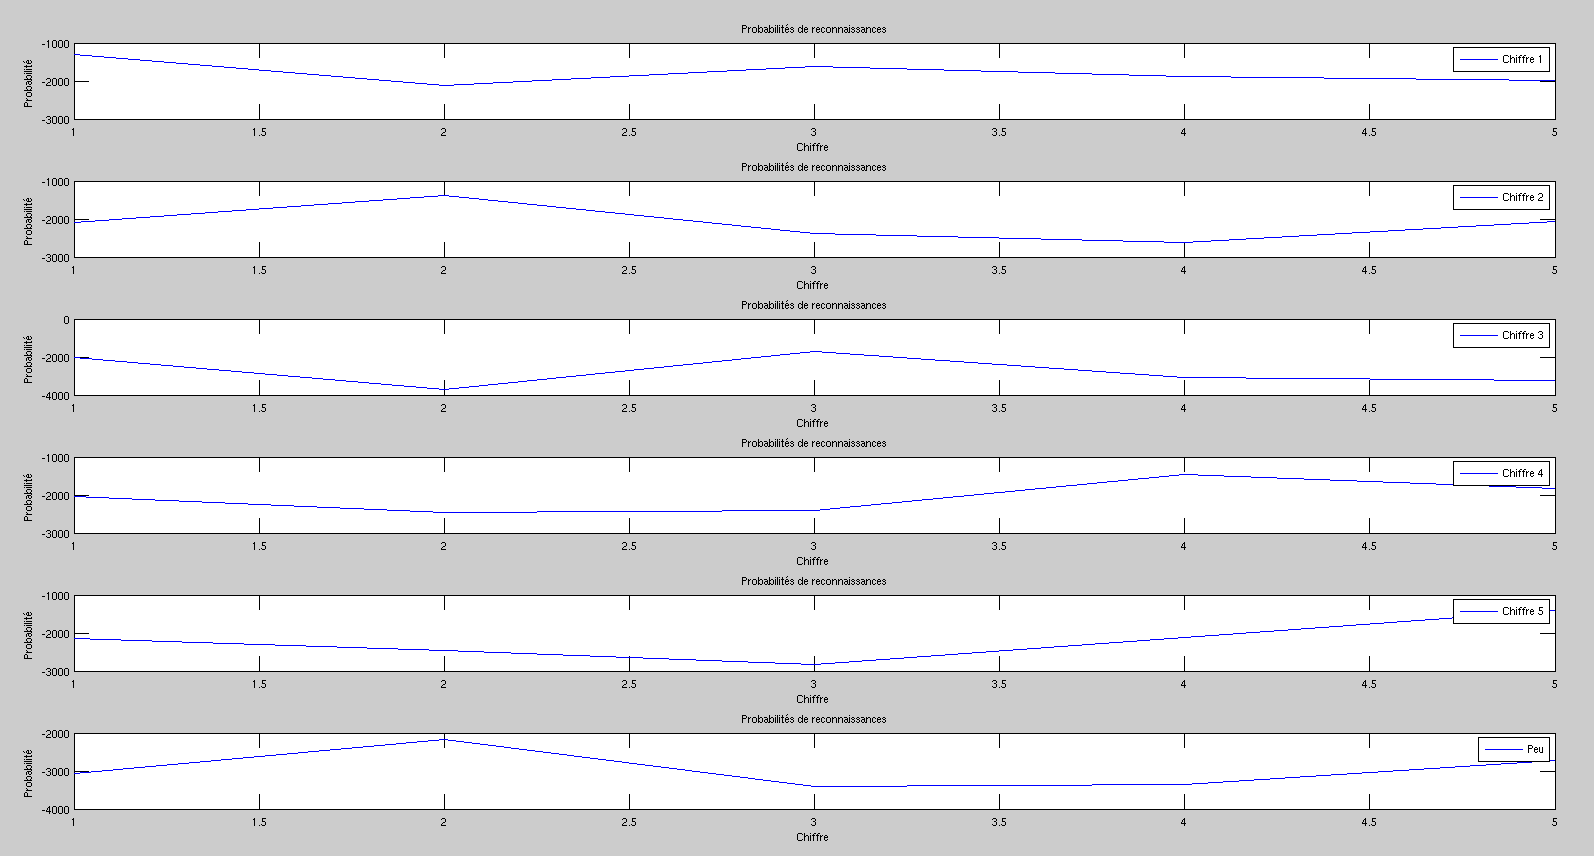
\includegraphics[width=17cm]{Ressources/Graphiques/ProbaReconnSepare.png} 
\end{center}

On peut voir dans le tableau ainsi que dans le graphique qui précède que chaque chiffre obtient la probabilité la plus élevée dans la HMM qui lui correspond. Ils sont donc tous bien reconnus.

\begin{center}
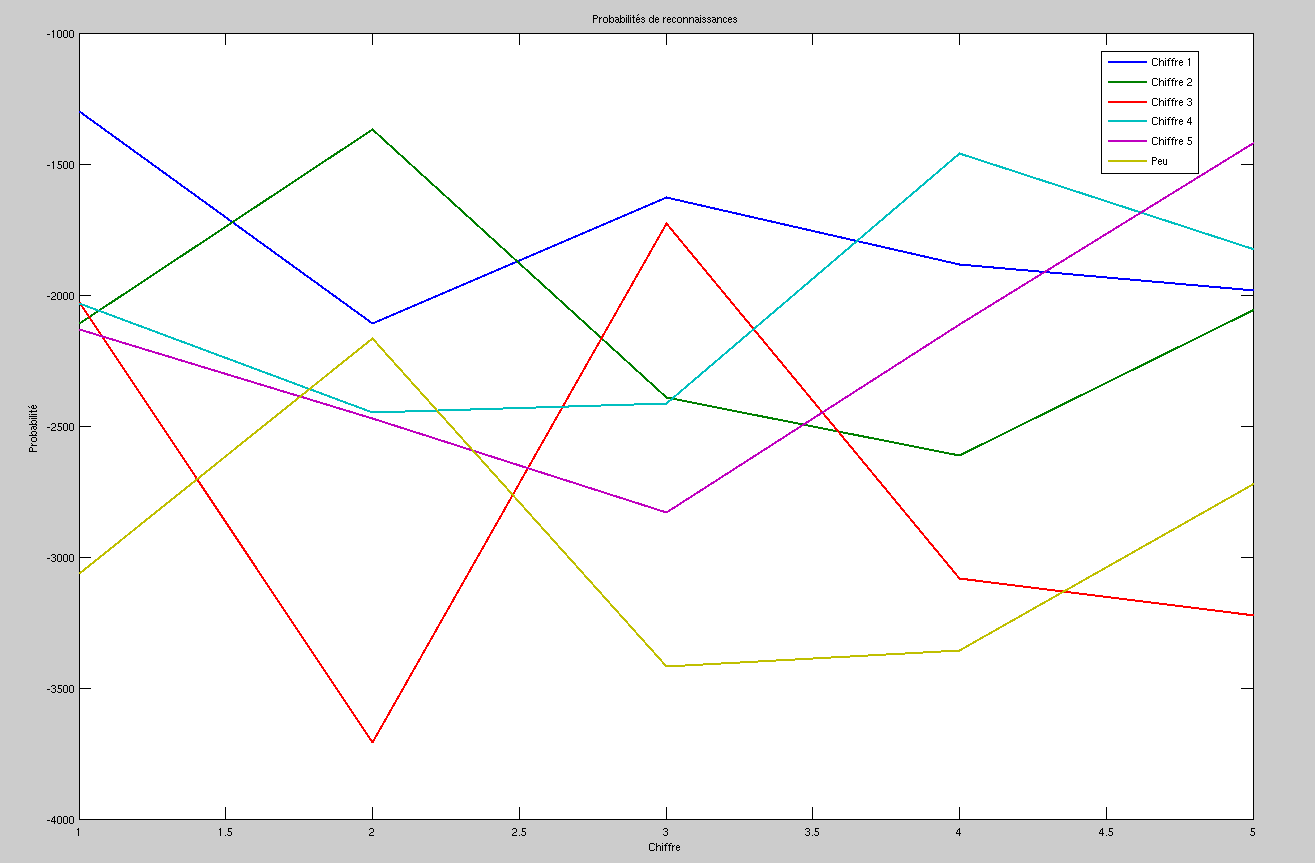
\includegraphics[width=12cm]{Ressources/Graphiques/ProbaReconnTout.png} 
\end{center}

On voit ici que la probabilité du mot peu est la plus haute pour le chiffre deux. Les mots peu et deux ont un profil très similaire.


\subsection{h) Demander à un collègue de vous fournir ses enregistrements de test et faites la reconnaissance sur ces fichiers avec vos modèles entraînés.}

Nous testons maintenant les HMM avec les échantillons de tests d'un collègue. Le but de cette manipulation est de voir si le fait d'entrainer les systèmes avec les enregistrements d'une personne et d'utiliser les enregistrements d'une autre personne dans les tests influence les résultats.
\\

\begin{tabular}{|c|c|c|c|c|c|}
\hline 
Chiffre testé & Proba un & Proba deux & Proba trois & Proba quatre & Proba cinq \\ 
\hline 
un & -2817.8 & -3342.6 & -2510.1 & -2736.2 & -2686.3 \\ 
\hline 
deux & -2680.6 & -2258.5 & -2365.4 & -2629.2 & -2271.5 \\ 
\hline 
trois & -3982.2 & -4891.9 & -2943.0 & -3758.6 & -3845.7 \\ 
\hline 
quatre & -3163.2 & -3269.7 & -3085.2 & -3051.4 & -2562.5 \\ 
\hline 
cinq & -3405.0 & -3385.6 & -3096.9 & -3013.2 & -2706.5 \\ 
\hline 
peu & -3786.7 & -2992.9 & -2460.4 & -2331.0 & -2713.4 \\ 
\hline 
\end{tabular} 
\\

\begin{center}
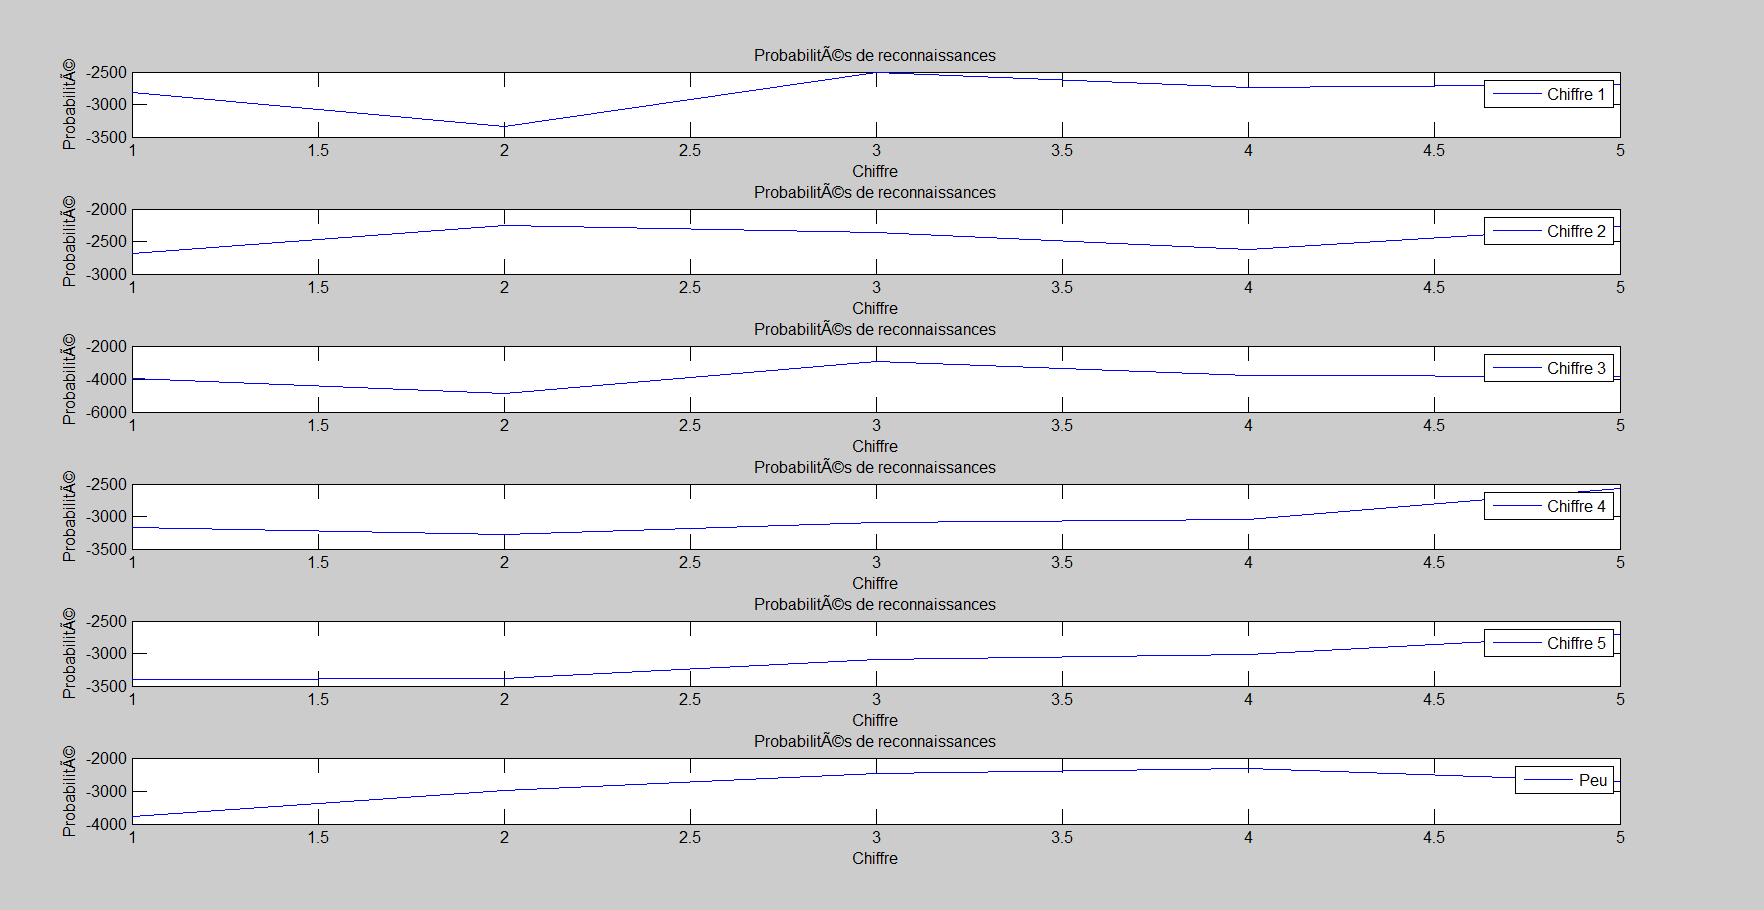
\includegraphics[width=17cm]{Ressources/Graphiques/ProbaReconnSepare_croise.png} 
\end{center}

On peut voir dans le tableau ainsi que dans le graphique qui précède que si l'on utilise les échantillons de tests d'une autre personne sur un système déjà entrainé, les mots ne sont pas tous reconnus correctement.

\begin{center}
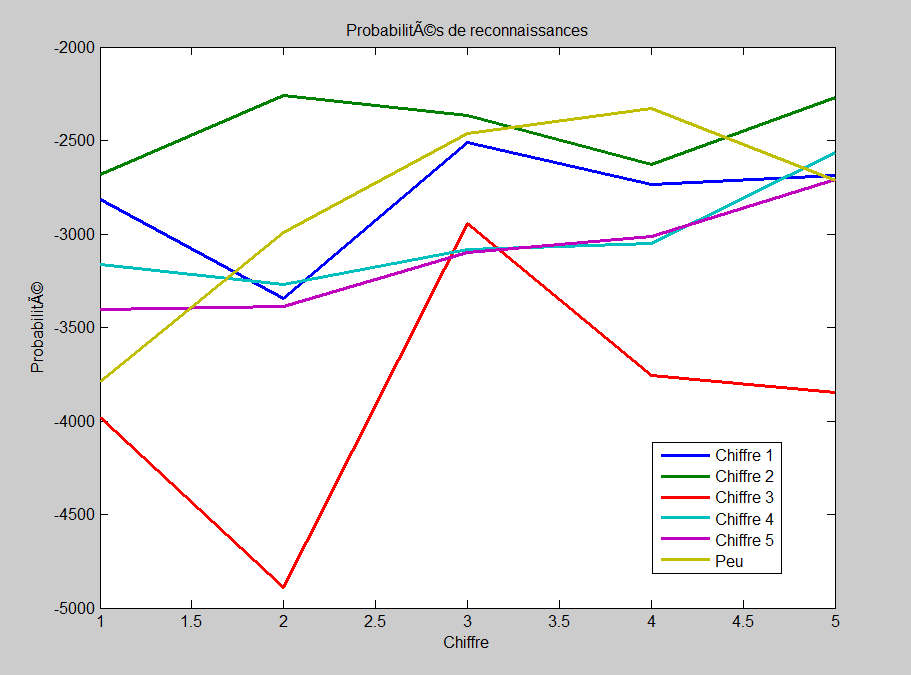
\includegraphics[width=12cm]{Ressources/Graphiques/ProbaReconnTout_croise.png} 
\end{center}

Dans notre cas, seuls les mots deux, trois et cinq sont reconnus correctement alors que les mots un et quatre sont faux. On peut aussi remarquer que, de manière générale, les courbes sont beaucoup plus lisses, la distinction entre chaque mots est donc moins bonne pour les HMM, les probabilité sont plus similaires.
\\
Puisque normalement, notre système devrait reconnaitre les mots et non pas la personne qui parle, nous pouvons conclure que le système devrait être entrainé avec plusieurs personnes et avec beaucoup plus d'échantillons pour avoir une fiabilité plus élevée.




